\section{There and back again}
In this section we will try to shed some light on the preliminary work that was done before we ended up on the path that lead to our project. It will consists of two parts. The first one will be a summary on our pre-project and the second one be early work with Voldemort.

\subsection{Energy efficiency of a Raspberry Pi cluster used for searching}
Our pre-project was split into three parts. Building a cluster of Raspberry Pis, building a search engine and then measure performance and power efficiency of our cluster compared to a Core i5 Macbook Pro. During the build we constructed our own power supply and built the frame holding the cluster along with network equipment. The search engine was written in C to be as fast as possible. We used an existing python program to create an index over a corpus of text documents, and used tf-idf for searching. Trough our performance testing we found that even though the Pis require a lot less energy to run, they are unable to keep up with modern hardware in a task so CPU demanding. It is worth mentioning that our entire corpus fit into memory, so a more disk based application could have seen very different results.

\begin{figure}[h]
    \centering
    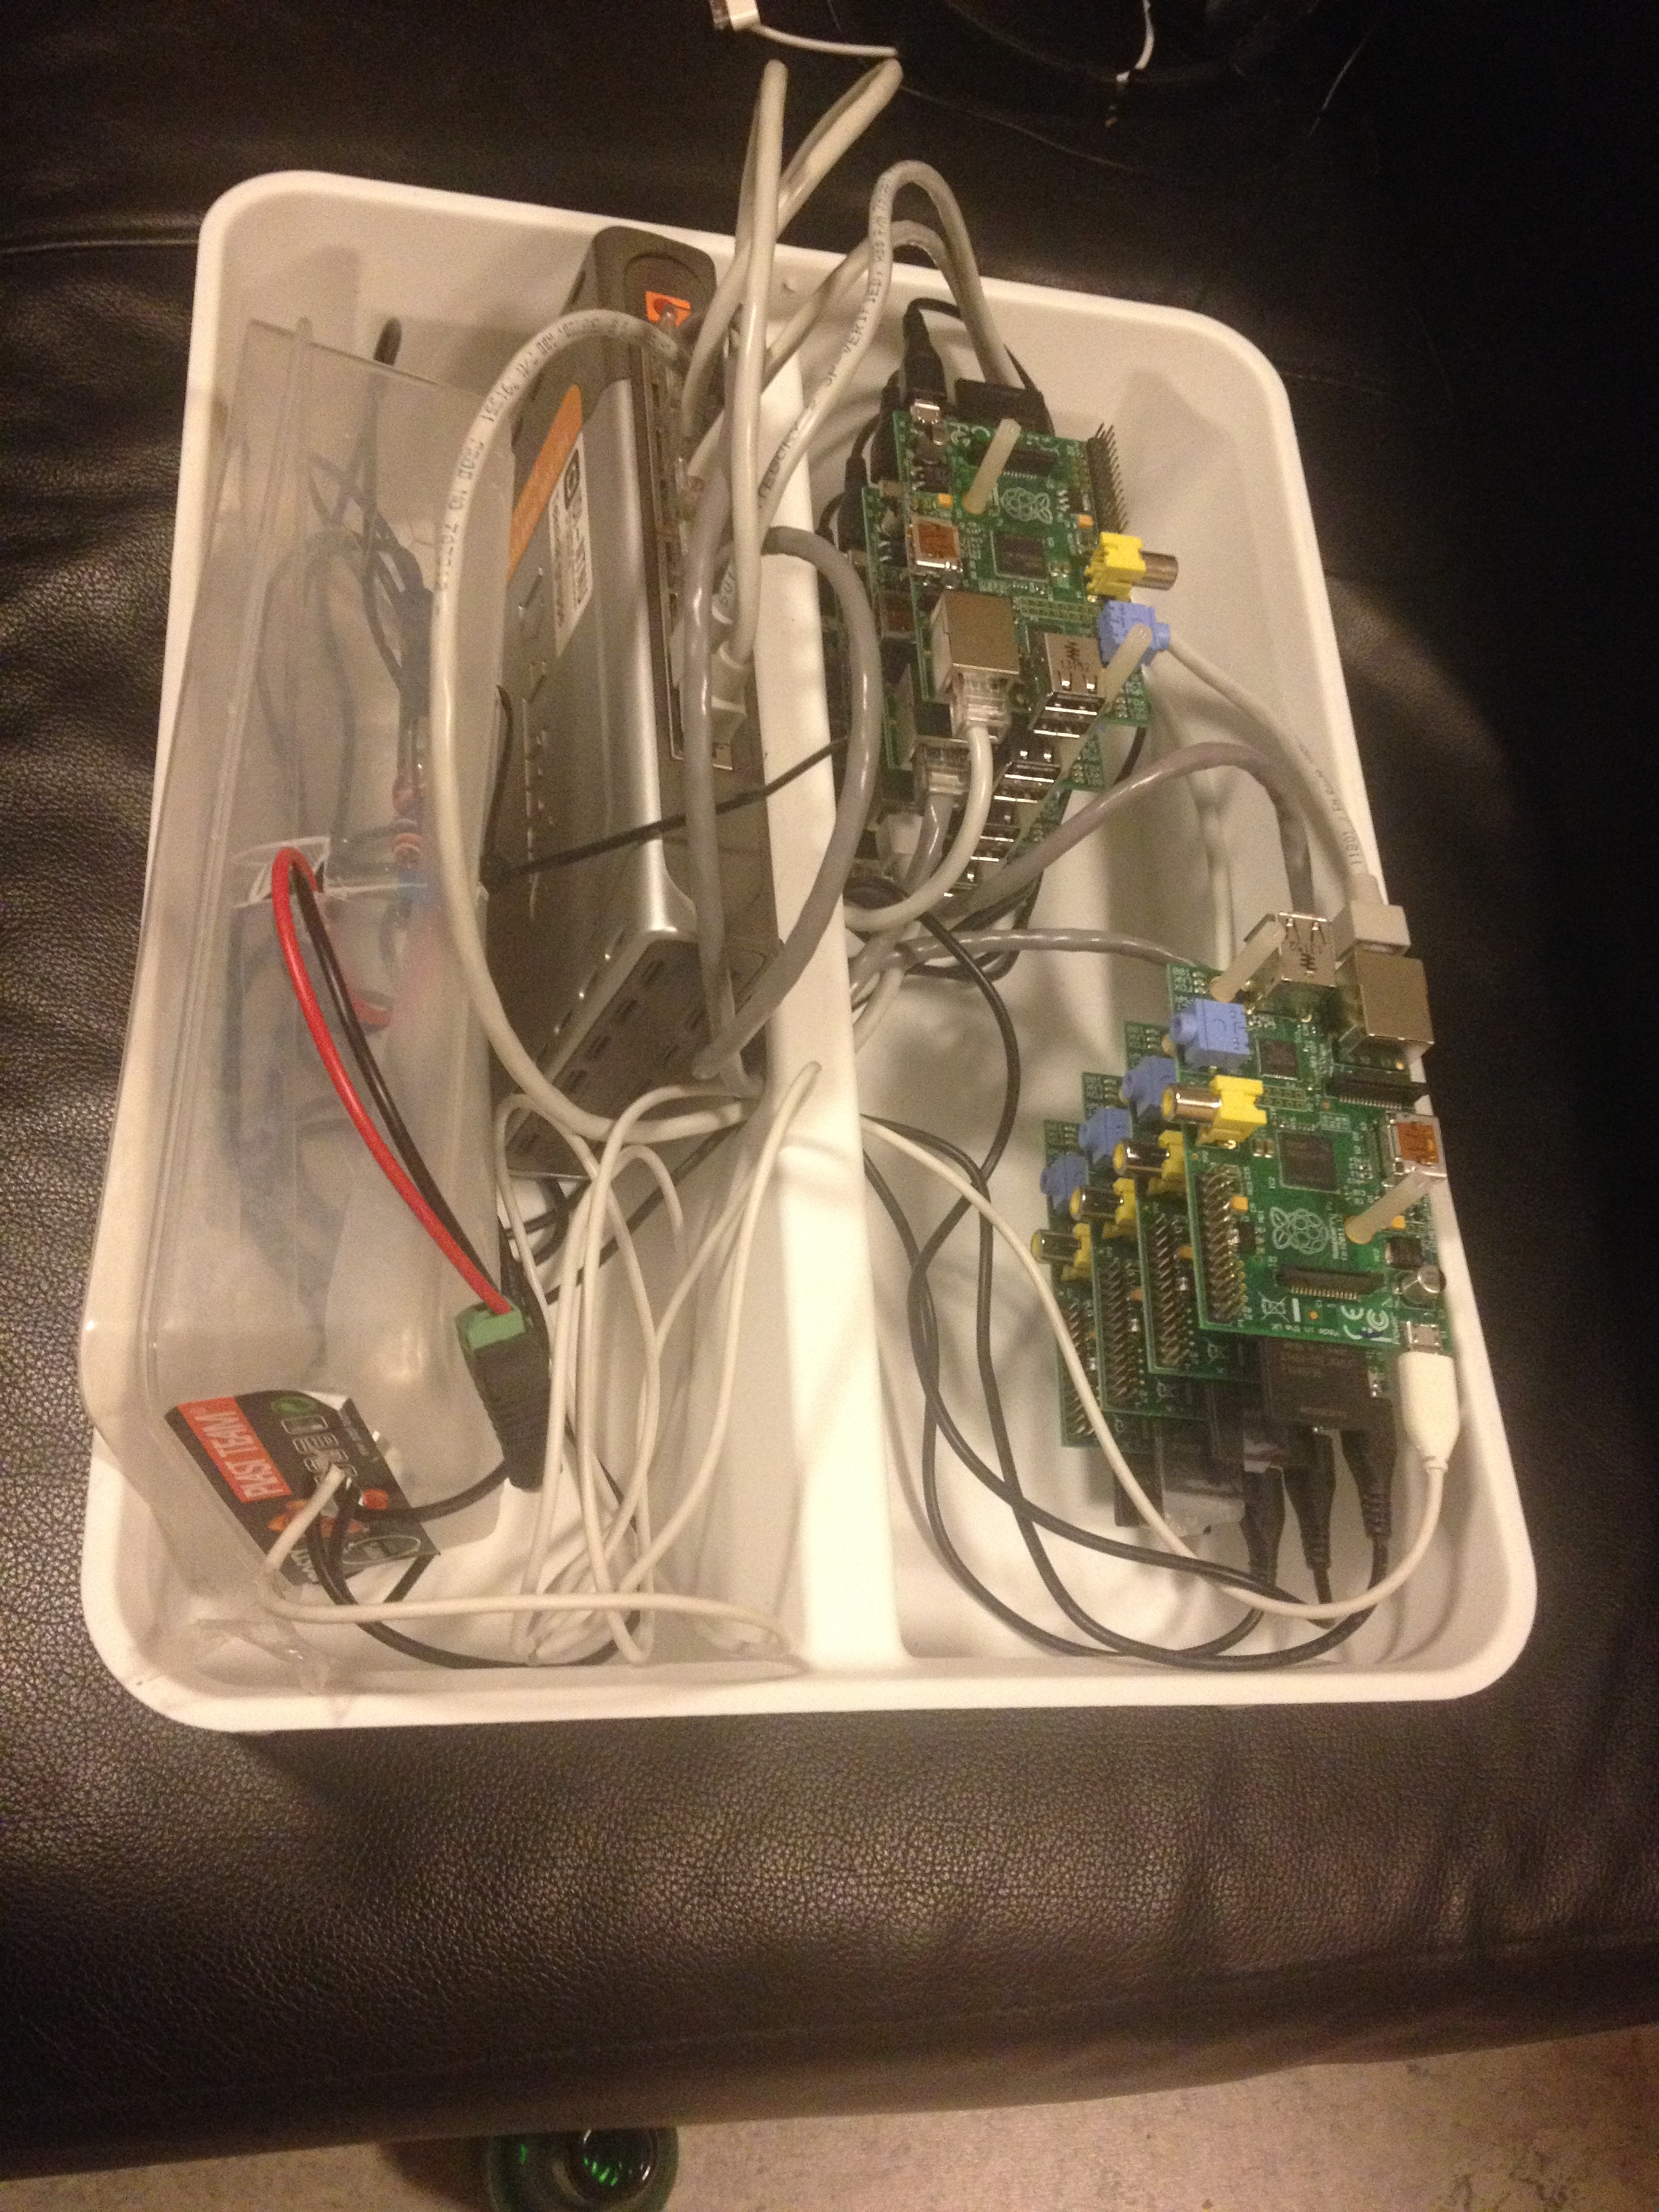
\includegraphics[width=0.5\textwidth]{thereandbackagain/cluster_beautiful.jpg}
    \caption{The Raspberry Pi cluster}
    \label{fig:cluster}
\end{figure}

\subsection{Early work with Raspberry Pis and Voldemort}
In the early days of our project we were planning to use our Raspberry Pi cluster to host a Voldemort service. However the limited memory of 512MB quickly turned out to be a problem. The Pis could run Voldemort without any problems until some of the background data exchange processes started and killed the JVM. After some debugging we determined that memory was a serious issue, and abandoned the idea of running Voldemort on our Pis. 

Now we had to find a more powerful cluster to run Voldemort for us. We decided to give virtual machines a try. We used an older Mac mini (mid 2010) with a 2.4 Ghz core duo processor and 8 GB worth of RAM, and created 4 virtual machines using VMware Fusion. They were all running Arch Linux with 1 GB memory. Initial tests quickly showed that we now had no issues with running out of memory. Although we now had a working setup, Mac mini was also being used as a media center, so we needed a more permanent solution. After querying the institute for a proper solution we were allowed access to 4 virtual machines running on a server within the institute. This is were the Voldemort cluster is running when we carried out our experiments. The server is running an Intel(R) Xeon(R) CPU E5-2650 0 @ 2.00GHz and each VM is provided 1 GB RAM.